\documentclass[crop=false]{standalone}
\usepackage{blindtext, mdframed, graphicx, float}

\begin{document}
\section*{I.U1 Slavné osobnosti fyziky}
K obrázkům níže přiřaďte jména vyobrazených fyziků a jejich přínos vědě (využijte pojmy z následujích rámečků).

\begin{mdframed}[frametitle={Jména}, frametitlealignment=\center, ]
    \begin{center}
        Albert~Einstein, Isaac~Newton, Michael~Faraday, Stephen~Hawking, Erwin~Schrödinger, Marie~Curie-Skłodowska
    \end{center}
\end{mdframed}
\vspace{-0,2cm}
\begin{mdframed}[frametitle={Díla}, frametitlealignment=\center]
    \begin{center}
        speciální~princip~relativity, gravitační~zákon, elektromagnetická~indukce, stanovení~teploty~černé~díry, myšlenkový~experiment~s~kočkou~v~krabici, teorie~radioaktivity
    \end{center}
\end{mdframed}

\begin{figure}[H]
  \minipage{0,2\textwidth}
    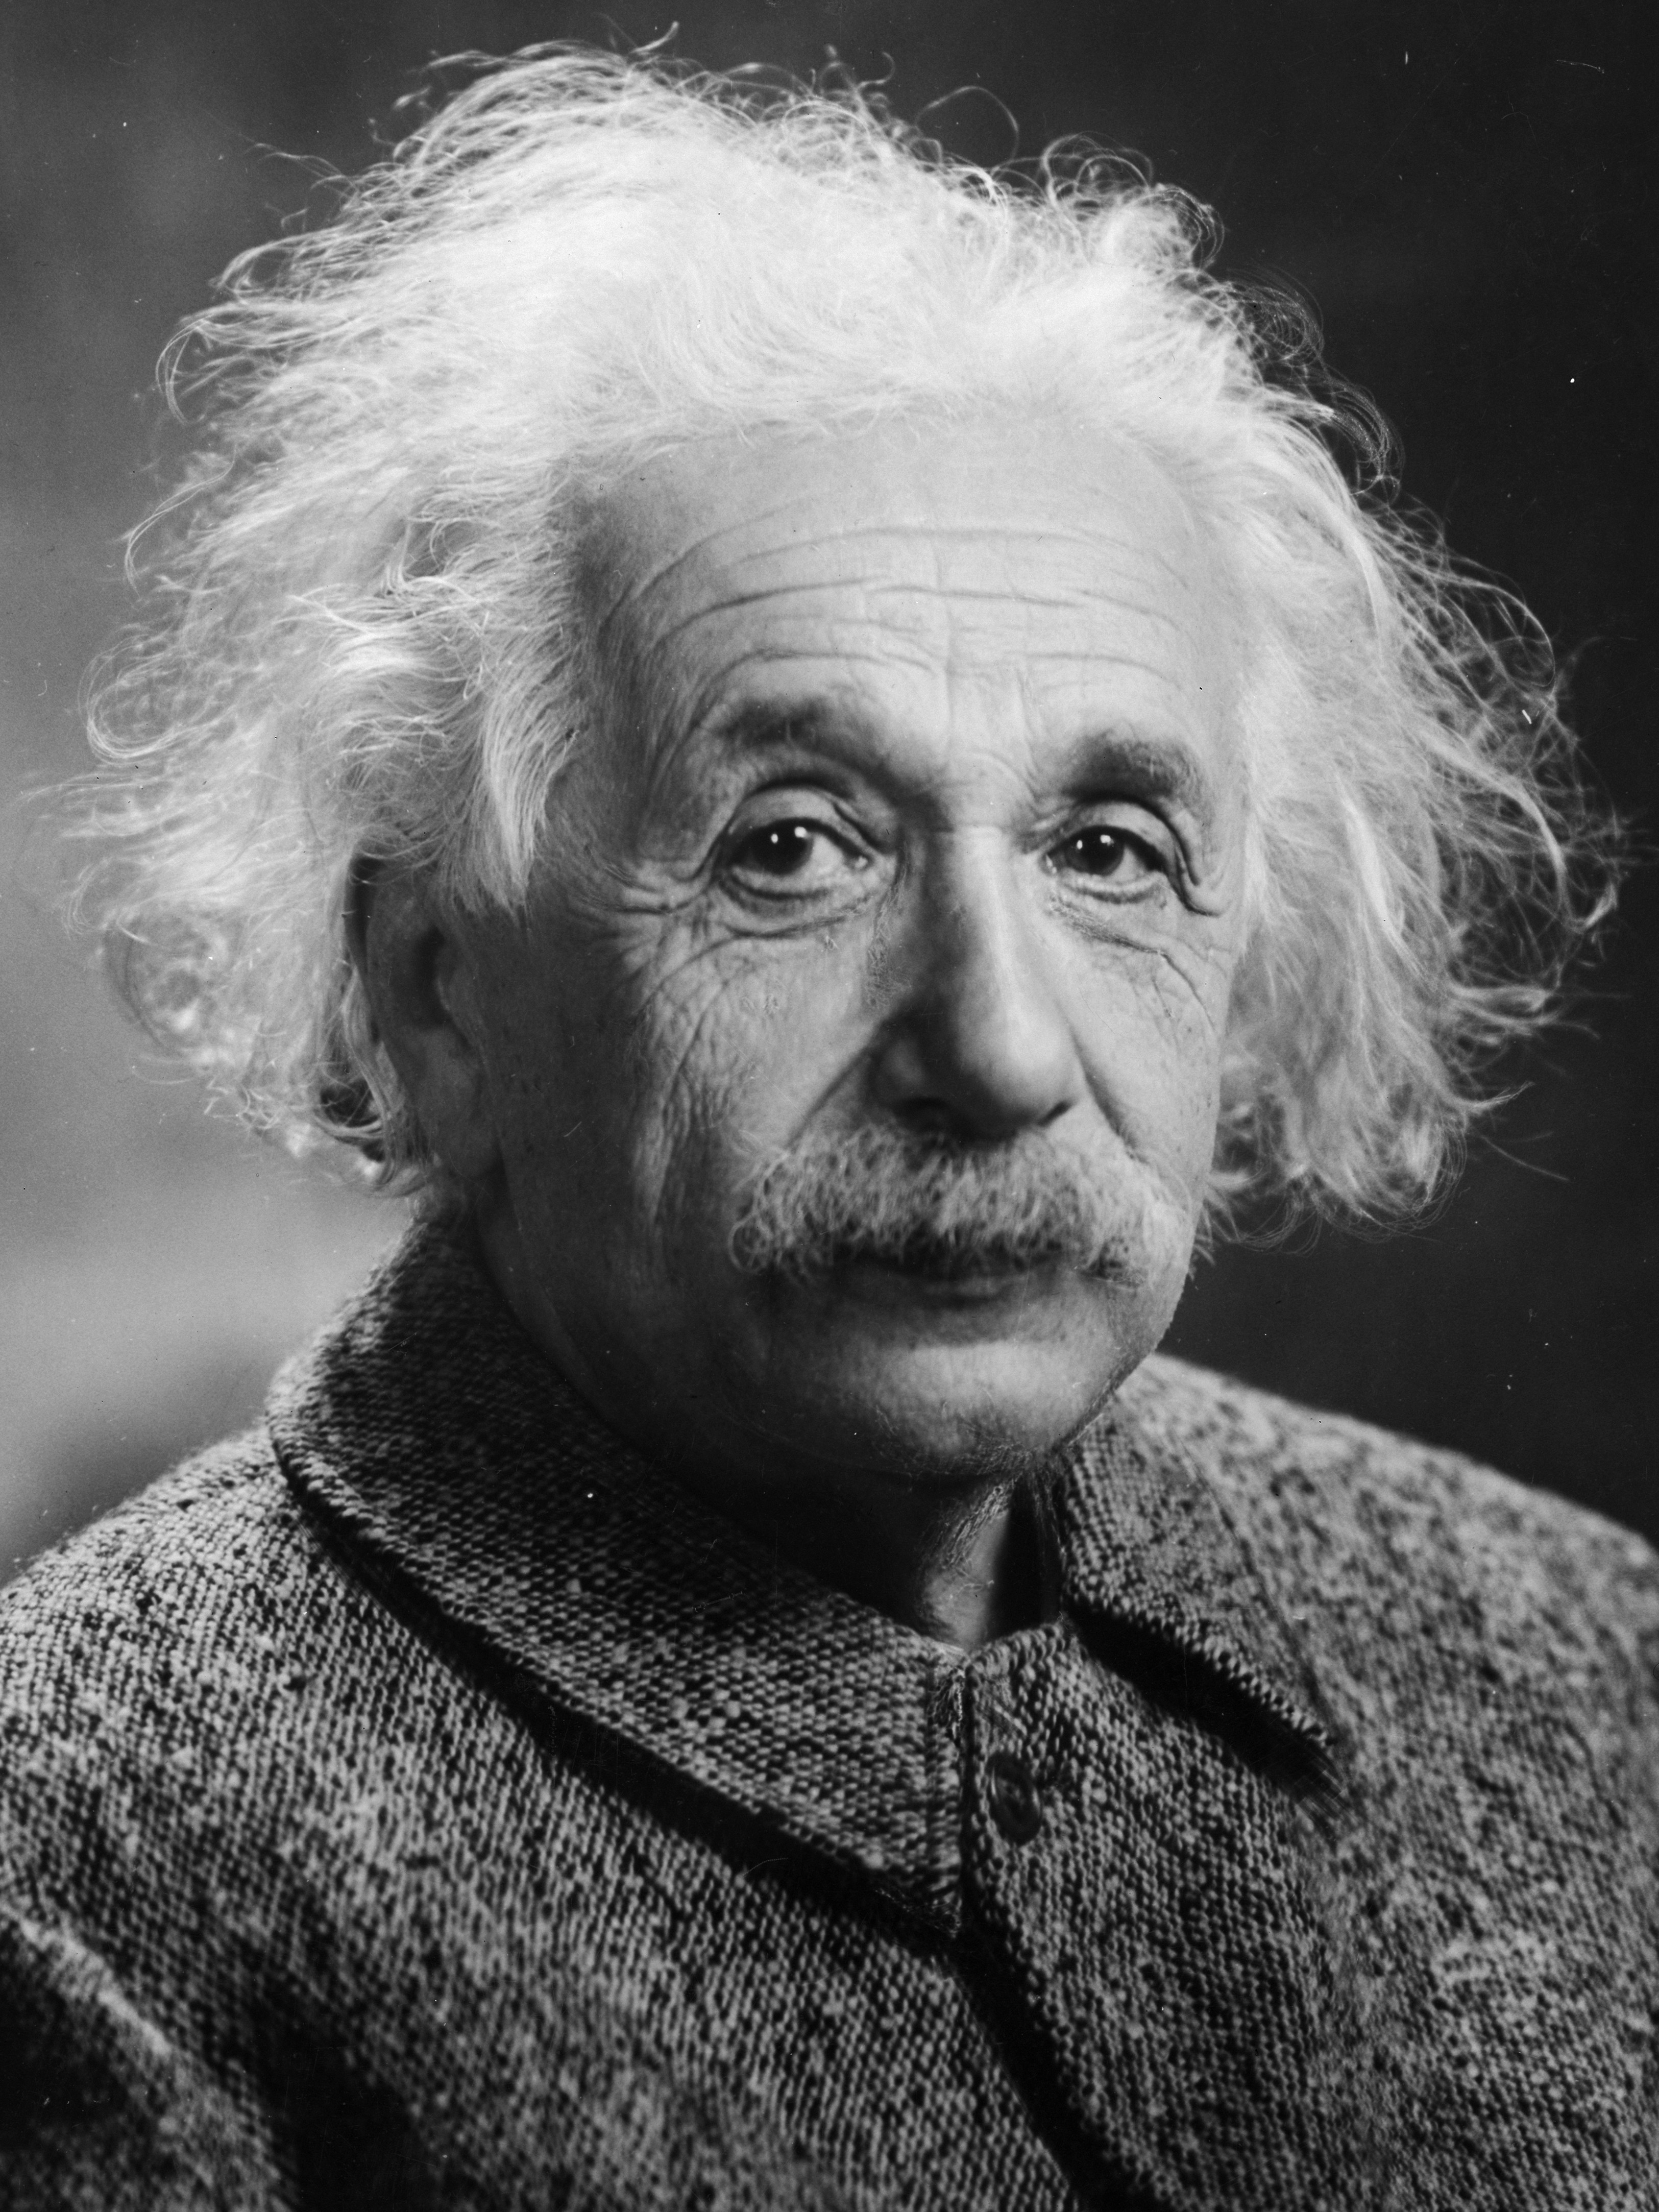
\includegraphics[width=\linewidth]{images/albert-einstein.jpeg}
    \begin{center}
      1
      \end{center}
  \endminipage\hfill
  \minipage{0.2\textwidth}
    \includegraphics[width=\linewidth]{images/erwin-schrödinger.jpg}
    \begin{center}
      2
      \end{center}
  \endminipage\hfill
  \minipage{0.2\textwidth}%
    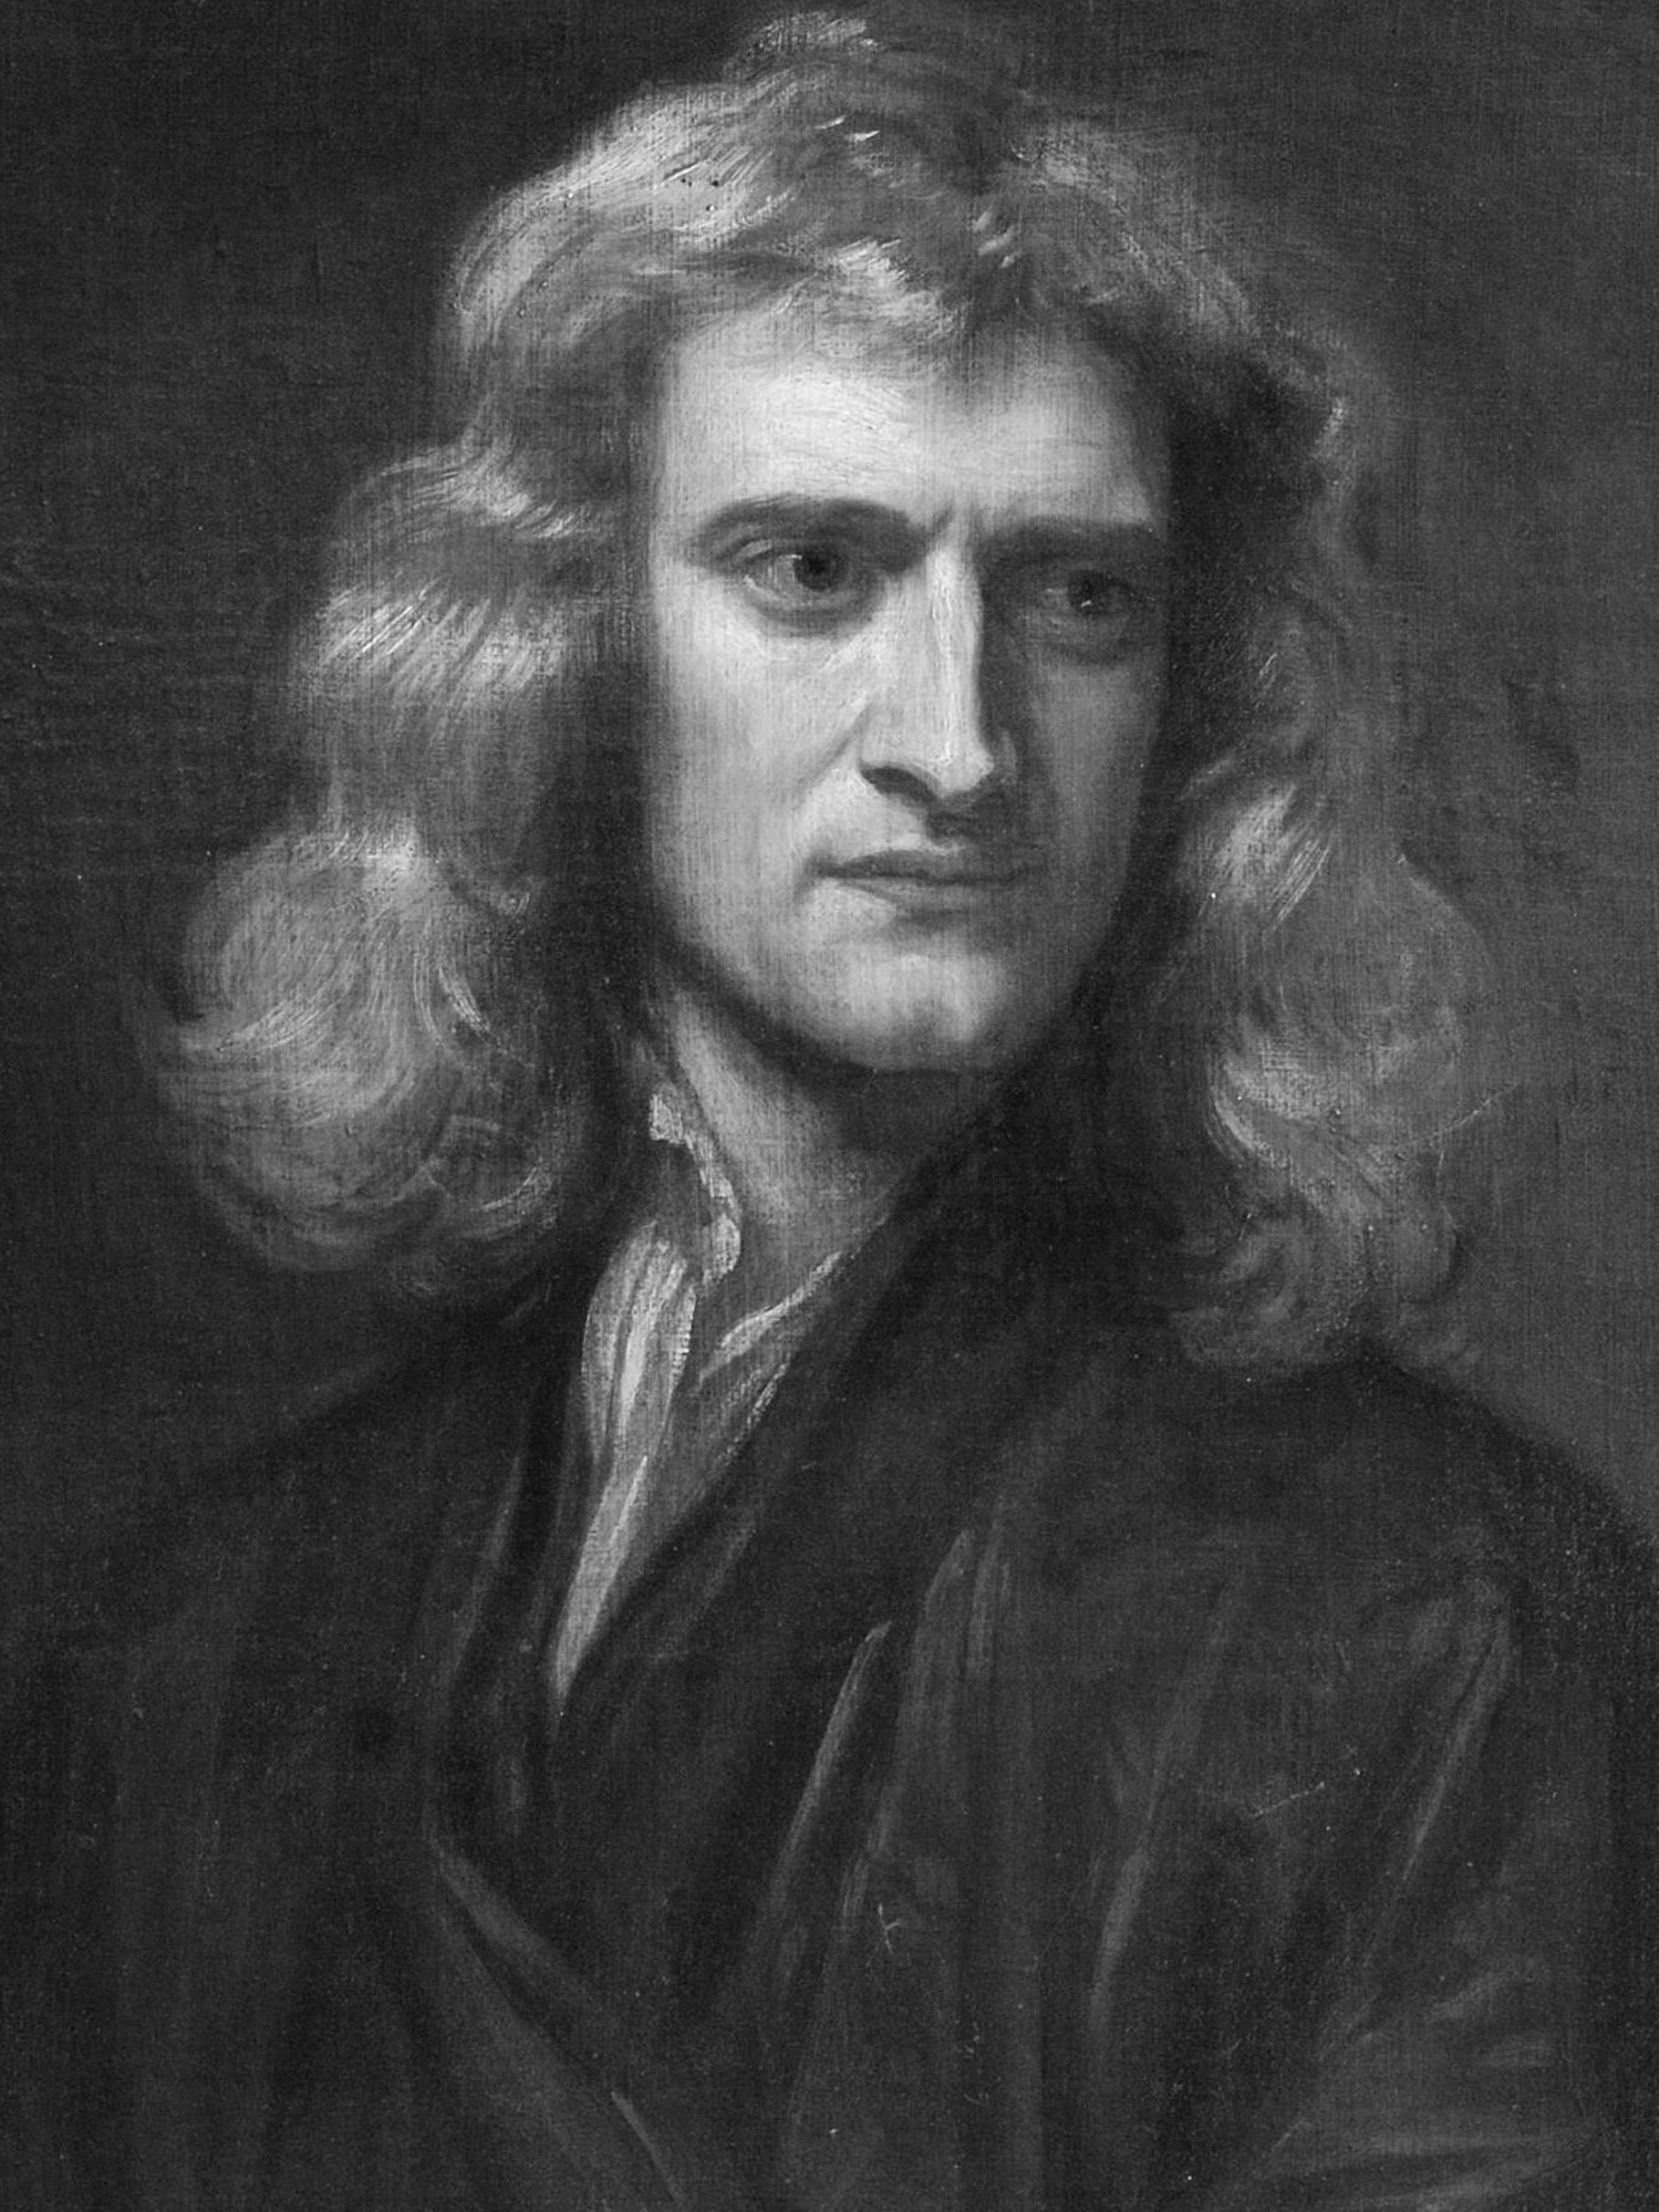
\includegraphics[width=\linewidth]{images/isaac-newton.jpg}
    \begin{center}
    3
    \end{center}
  \endminipage
\end{figure}

\begin{figure}[H]
  \minipage{0.2\textwidth}
    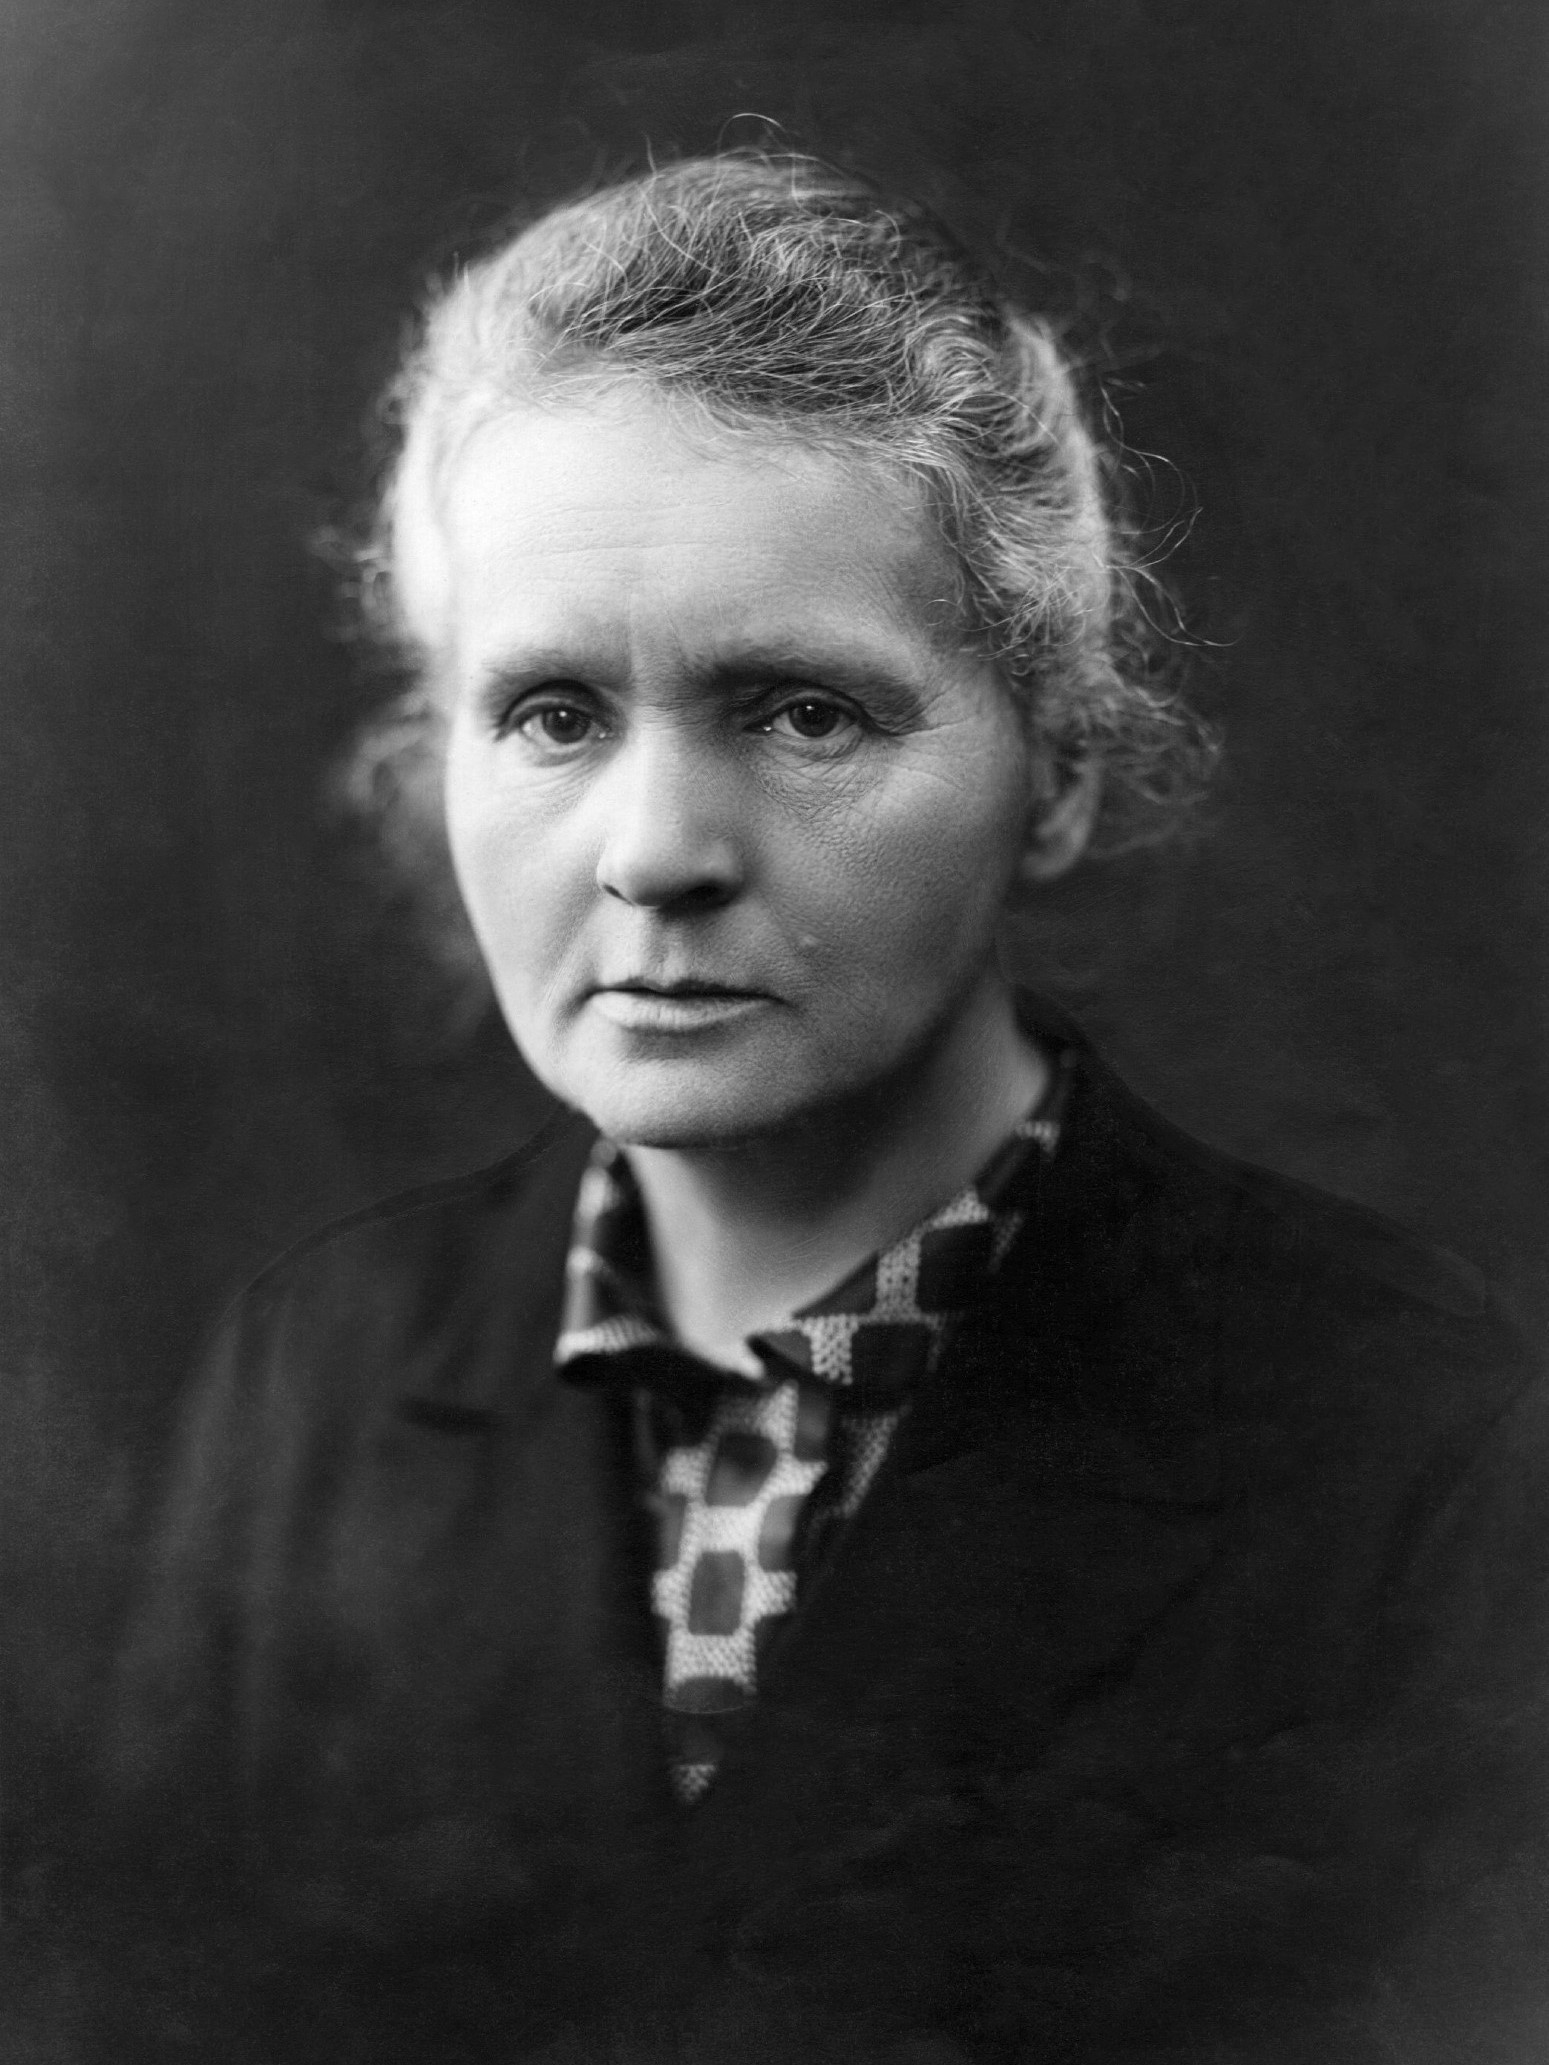
\includegraphics[width=\linewidth]{images/marie-curie-sklodowska.jpg}
    \begin{center}
      4
      \end{center}
  \endminipage\hfill
  \minipage{0.2\textwidth}
    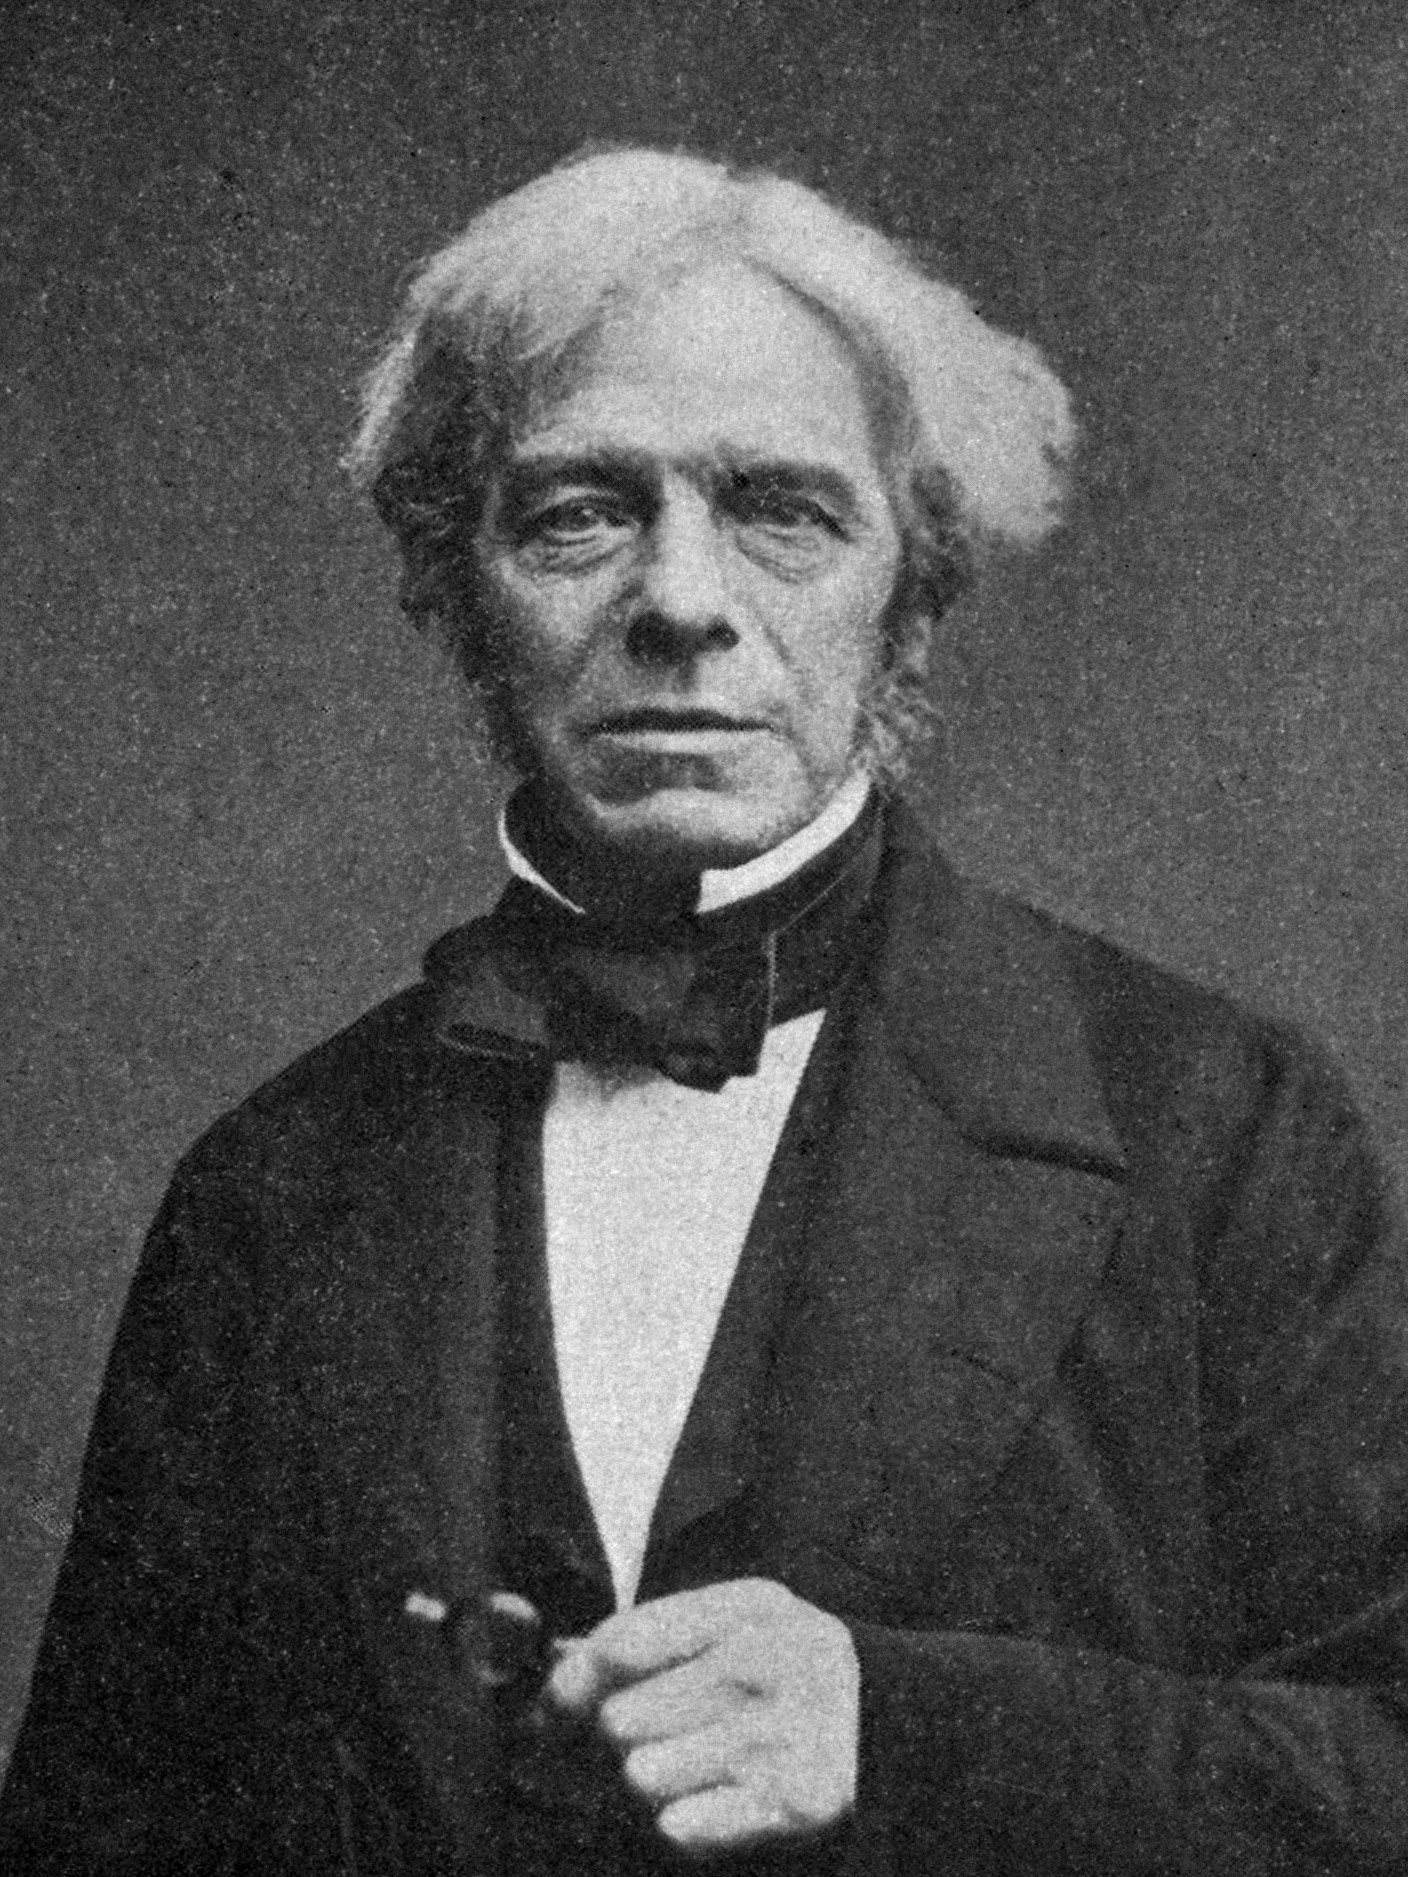
\includegraphics[width=\linewidth]{images/michael-faraday.jpeg}
    \begin{center}
      5
      \end{center}
  \endminipage\hfill
  \minipage{0.2\textwidth}%
    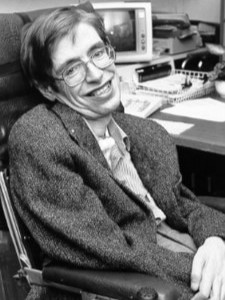
\includegraphics[width=\linewidth]{images/stephen-hawking.jpg}
    \begin{center}
      6
      \end{center}
  \endminipage
\end{figure}

\end{document}
